\section{Introduction}

Huge amounts of resources are used every year to build and maintain roads
around the globe. The Swedish Road Administration alone, has a annual budget
of 21 billion SEK \cite{vagverket}. Reducing traffic jams, and thereby
reducing the need for building new roads is highly motivated.\\\\

\begin{figure}[H]
    \begin{center}
    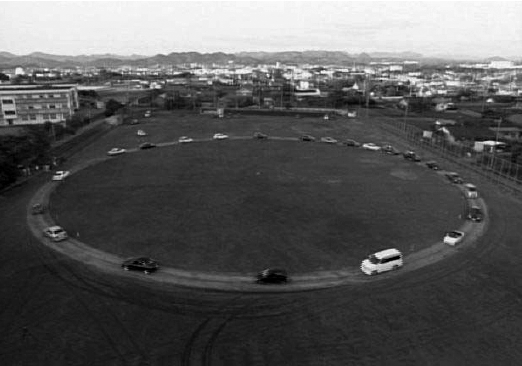
\includegraphics[width=0.75\textwidth]{sug_circlephoto.png}
    \caption{\label{sug_photo}
Experiment by Y. Sugiyama el al. \cite{sugiyama}. 22 cars on a circular road
of length 230 m. A traveling phantom jam has appeared and can now bee seen in
the upper-right part of the photo.
} \end{center} \end{figure}

In free flowing traffic, traffic jams can appear for no apparent reason. Even
without the presence of bottle-necks such as traffic-lights, crossroads or
slip roads. In light traffic, drivers adjust to any
instabilities, but as soon as traffic reaches a certain level of density, jams
occur. This phenomena is known as jamitons or \emph{phantom jams} and has
recently been confirmed experimentally by Y. Sugiyama et al. (see fig
\ref{sug_photo} and \ref{sug_positions}) \cite{sugiyama}. Once a phantom jam has been
established, the jam travels backwards in traffic as a wave. Recently it was
shown by M. R. Flynn et al. \cite{mit} that these waves are mathematically
similar to travelling shock-waves caused by explosions.\\\\

\begin{figure}[H]
    \begin{center}
    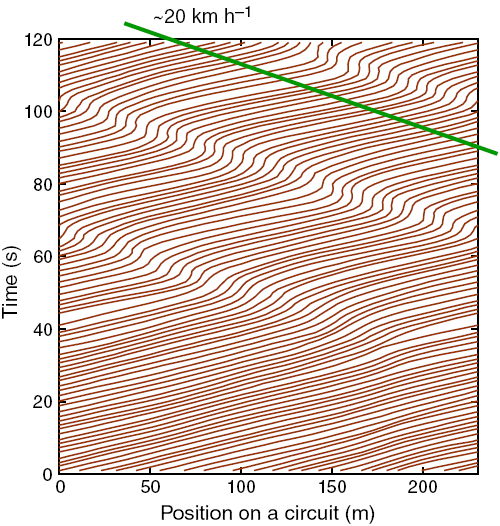
\includegraphics[width=0.6\textwidth]{sug_positions.png}
    \caption{\label{sug_positions}
Data measured during the experiment seen in fig \ref{sug_photo}. A disturbance
can be seen after 40 s and is quickly amplified into a phantom jam, travelling
backwards around the circle at approximately 20 km/h.
Diagram by Y. Sugiyama el al. \cite{sugiyama}.}
\end{center} \end{figure}

Traffic flow and thereby the efficiency of roads, is severely reduced by
traffic jams such as phantom jams (see fig \ref{sug_flow}) \cite{sugiyama}. If we implement a system that shifts the critical level of traffic density at which phantom jams occur upwards, we improve road efficiency. In this report we evaluate two such systems: Adaptive Cruise Control and an improved version that we have named Enhanced Adaptive Cruise Control. Results are taken from our simulator based on agent-based modelling.

\begin{figure}[H]
    \begin{center}
    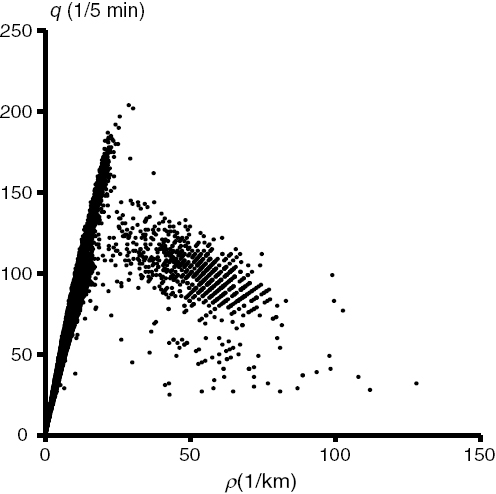
\includegraphics[width=0.6\textwidth]{sug_trafficFlow.png}
    \caption{\label{sug_flow}
Traffic flow as a function of traffic density. The data is clearly divided
into two sets, one representing free flowing traffic and the other (above the
threshold of 25 vehicles per km) representing congested traffic (with traffic
jams).  Results from article by Y. Sugiyama el al. \cite{sugiyama}.  Data was
measured by Japan Highway Public Cooperation on Japanese highways. Similar
observations have been made in many places and seems to be almost a universal
property of highway traffic.}
    \end{center}
\end{figure}

